% Created 2021-09-21 Tue 18:34
% Intended LaTeX compiler: pdflatex
\documentclass[11pt]{article}
\usepackage[utf8]{inputenc}
\usepackage[T1]{fontenc}
\usepackage{graphicx}
\usepackage{grffile}
\usepackage{longtable}
\usepackage{wrapfig}
\usepackage{rotating}
\usepackage[normalem]{ulem}
\usepackage{amsmath}
\usepackage{textcomp}
\usepackage{amssymb}
\usepackage{capt-of}
\usepackage{hyperref}
\usepackage{awesomebox}
\usepackage{booktabs}
\usepackage{placeins}
\usepackage{siunitx}
\usepackage{minted}
\usepackage{cleveref}
\usepackage{tikz}
\usetikzlibrary{backgrounds,matrix,fit,calc}
\usepackage{pgfplots}
\pgfplotsset{compat=1.16}
\definecolor{metropolisorange}{RGB}{235,129,27}
\author{Mattia Gazzola}
\date{}
\title{Project 1: Evolutionary Optimization Algorithms\\\medskip
\large ME498: Computational modeling and optimization}
\hypersetup{
 pdfauthor={Mattia Gazzola},
 pdftitle={Project 1: Evolutionary Optimization Algorithms},
 pdfkeywords={},
 pdfsubject={},
 pdfcreator={Emacs 28.0.50 (Org mode 9.3.6)},
 pdflang={English}}
\begin{document}

\maketitle
\pgfplotsset{
colormap={whitered}{color(0cm)=(white); rgb255(1cm)=(235,129,27)}
}

\textbf{Issue Date} : \today

\textbf{Teaching Assistant} : Tejaswin Parthasarathy, \texttt{tp5@illinois.edu}

\textbf{Submission Date/Time}: Friday 11:59 PM, 22 October, 2021

\textbf{Submission Instructions}:
\begin{itemize}
\item You need to submit both your presentation (as \texttt{.pdf}, \texttt{.ppt[x]} or \texttt{.key}) and code
(as \texttt{.py} or \texttt{.ipynb}) on Compass, in separate links
\item Submit your code file(s) packaged as a \texttt{.zip} or \texttt{.tar.gz} files (please do not use
\texttt{.7z} or other formats) and name the compressed file as \texttt{<net\_id>\_code\_01}
\item Submit your presentation file(s) packaged as a \texttt{.zip} or \texttt{.tar.gz} files (please do not use
\texttt{.7z} or other formats) and name the compressed file as \texttt{<net\_id>\_slides\_01}
\item If you are working in a group, its sufficient if \textbf{one} member of the group submits both the code
and slides. It goes without saying that this submission (both code and presentation) should
contain the names of \textbf{all} group members (as comments in the code and as subtitles in the
slides).
\end{itemize}

\section{Guidelines}
\label{sec:orgf8caca7}
General advice that pertains to all the problems include:
\begin{enumerate}
\item Pick sensible representation, fitness function, selection and mutation
operators and parameters wherever applicable.
\item Remember to present (during the project evaluation) the motivation for the
algorithmic design choices you have made\ldots{}
\item Explore as much as possible---change parameters, selection/mutation
operators etc\ldots{} We want you to learn how the optimizer ``thinks'' and works.
\item We will evaluate your work based on your understanding and findings, and
not on the code quality. However since you are learning \texttt{Python}, it is
always a good idea to code efficiently. Use canned algorithms in \texttt{numpy} or
\texttt{scipy} wherever possible.
\item You are free to consult any material you want (including but not limited to
\cref{sec:references}). However you are expected to follow the Student Code
on academic integrity---plagiarism will not be tolerated!
\end{enumerate}

\section{The Knapsack problem}
\label{sec:org23ab825}
\subsection{Definition}
\label{sec:orgbe35753}
  Use genetic algorithm and rank-\(\mu\), weighted recombination version of the CMA
evolutionary strategy discussed in class to find the solution to the \textbf{0/1 variant} of
the Knapsack problem.
\subsection{Details}
\label{sec:org8adf41d}
More details about the 0/1 Knapsack problem are contained in the lecture slides.
Alternatively, the \href{https://en.wikipedia.org/wiki/Knapsack\_problem}{Wikipedia} page also has a lot of information about this
problem. Quoting the introductory text,
\begin{quote}
`` The knapsack problem or rucksack problem is a problem in combinatorial
optimization: Given a set of items, each with a weight and a value, determine
the number of each item to include in a collection so that the total weight is
less than or equal to a given limit and the total value is as large as possible.
It derives its name from the problem faced by someone who is constrained by a
fixed-size knapsack and must fill it with the most valuable items. ''
\end{quote}

Your task is to find an optimal distribution of items to carry, that
maximizes the overall value while adhering to the weight limit, using both
\begin{itemize}
\item GA
\item CMA
\end{itemize}
and compare the performance of these algorithms on this function. Details about
the dataset for this problem is given below in \cref{sec:data}. Note that this is a constrained
optimization problem and your design choices in the
algorithm need to reflect this. As this seems like a problem with integer
solutions, consider how you can change CMA to reflect this property. As we are
interested in black-box optimization algorithms, we assume we do not know
anything about the problem structure. This means that using a randomly generated
population around \(\mathbf{x}_0 =\mathbf{0}\)---the vector of zeros---to
initialize the algorithm is a good idea.

Finally, after answering all the questions above and implementing your
algorithm, explore the design choices (be it parameters or operators) on the
performance of the algorithms.
\subsection{Data}
\label{sec:data}
There are two data sets--A, B. Each data set will be posted on Compass as
simple \texttt{numpy npz} files with the knapsack capacity (total weight of the
knapsack), number of different items (which are all assumed to be distinct in
the 0/1 knapsack problem so you \textbf{do not} need to worry about \emph{choosing} same
items), and their values + weights. For convenience you can read the
information using \texttt{numpy}'s \texttt{load} function, shown in the snippet below:

\begin{minted}[]{python}
import numpy as np

# Load data from npz file
my_data = np.load('file_name.npz')

# Data stored as a dictionary
# use data however you want
bag_capacity = my_data['capacity']
'''
other possible keys include
capacity : Bag capacity in terms of total weight, float
n_items : Number of items, integer value
item_values : Value of each item, a (n_items, ) numpy array
item_weights : Weight of each item, a (n_items, ) numpy array
'''

\end{minted}

\section{Minima of the parabola}
\label{sec:org531371d}
\subsection{Definition}
\label{sec:org1cb1152}
  Use genetic algorithm and rank-\(\mu\), weighted recombination version of the CMA
evolutionary strategy discussed in class to find the minima of a simple parabola.
\subsection{Details}
\label{sec:orgbd4bf86}
The one-dimensional parabola is a continuous, convex, unimodal function. We
pick the parabola given by the formula
\begin{equation}
f(x) = 10 \cdot x^2
\end{equation}

Your task is to find the optimum of this function using
\begin{itemize}
\item GA
\item CMA
\end{itemize}
and compare the performance of these algorithms on this function.
Furthermore, explore the effect of the parameters (particularly in GA) on the
performance of the algorithms. Start your search using a randomly initialized population around \(\mathbf{x}_0 = \mathbf{0}\)---the vector of zeros.
\section{Minima of the Rotated Hyper-Ellipsoid}
\label{sec:org27d6940}
\subsection{Definition}
\label{sec:org1344c1a}
  Use genetic algorithm and rank-\(\mu\), weighted recombination version of the CMA
evolutionary strategy discussed in class to find the minima of the
two-dimensional rotated ellispoid.
\subsection{Details}
\label{sec:orge64b6d1}
The two-dimensional Rotated Hyper-Ellipsoid is a continuous, convex, unimodal
and non-separable function. We pick the variant that is rotated \(\frac{\pi}{6} \; \si{rad}\) clockwise from the \(x_1\)-axis and shifted along
both axes, given by the formula below:

\begin{equation}
f(\mathbf{x}) = \left( \dfrac{\sqrt{3}}{2} (x_1 - 3) + \dfrac{1}{2} (x_2 - 5) \right)^2 + 5 \cdot \left(  \dfrac{\sqrt{3}}{2} (x_2 - 5) - \dfrac{1}{2} (x_1 - 3)  \right)^2
\end{equation}


Graphically, it's contour plot is depicted in \cref{ellipsoid} for several
  values of \(c\).
\begin{figure}[h!]
\begin{center}
	\begin{tikzpicture}[
		declare function={shiftedellipsoid=0.25*(3^0.5*(x-3)+(y-5))^2 + 5*0.25*(3^0.5*(y-5)-(x-3))^2;}, scale=1.0]
		\begin{axis}[
			width=0.8\textwidth,
			view={0}{90},
			enlargelimits=false,
			grid=major,
			domain=-2:8,
			y domain=0:10,
			xlabel=$x_1$,
			ylabel=$x_2$,
		]
		\addplot3 [contour filled={levels={1,5,10,15,20,35,50, 100, 200, 400},labels=false},
        thick,samples=50,samples y=50] {shiftedellipsoid};
		\addplot3 [contour gnuplot={levels={1,5,10,15,20,35,50,100, 200, 400},labels=false,draw color=black},
        thick,samples=50,samples y=50] {shiftedellipsoid};
		\addplot [mark=*,
		mark size=2.5pt, metropolisorange, mark options={fill=metropolisorange}] coordinates {(3,5)};
		\end{axis}
	\end{tikzpicture}
\end{center}
\caption{The rotated hyper-ellipsoid in two dimensions, the horizontal axis corresponds to \( x_1 \) and the vertical to \( x_2 \)}
\label{ellipsoid}
\end{figure}


Your task is to find the optimum of this function using
\begin{itemize}
\item GA
\item CMA
\end{itemize}
and compare the performance of these algorithms on this function. Furthermore,
explore the effect of the parameters on the performance of the algorithms.
Start your search using a randomly initialized population around \(\mathbf{x}_0 = \mathbf{0}\)---the vector of zeros.

\section{Minima of the Rastrigin function}
\label{sec:org54c362f}
\subsection{Definition}
\label{sec:orgd51ea11}
  Use the rank-\(\mu\), weighted recombination version of the CMA
evolutionary strategy discussed in class to find the minima of the shifted
\emph{Rastrigin} function in two and five dimensions.

\subsection{Details}
\label{sec:orgffb5715}
The (unshifted) Rastrigin function is shown in \cref{rastr} for the case of two-dimensions.

\begin{figure}[htbp]
\centering
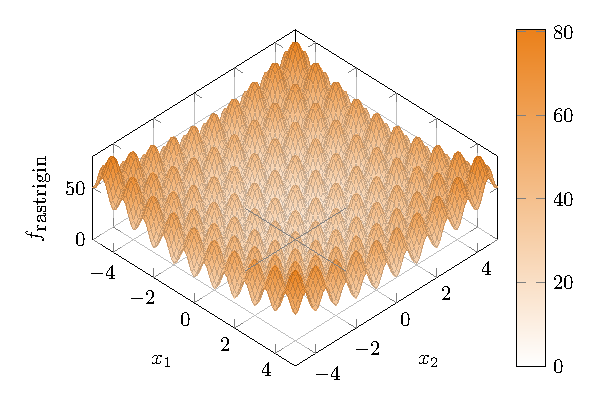
\includegraphics[width=0.9\textwidth]{images/shifted_rastrigin.pdf}
\caption{\label{rastr}The (shifted) Rastrigin function in two dimensions}
\end{figure}


It is a multi-modal function with several regularly distributed local minima,
and can be generalized to arbitrary dimensions using the analytical formula
shown below, for the shifted variant (which you should use as the objective
function):

\begin{equation}
f(\mathbf{x}) = 10d + \sum_{i=1}^{d} \left[ (x_i - 2)^2 - 10 \cos\left(2 \pi (x_i - 2) \right) \right]
\end{equation}
where \(d\) is the number of dimensions.


You need to find the local minima for this function in
\begin{itemize}
\item two dimensions ( \(d = 2\) )
\item five dimensions ( \(d = 5\) )
\end{itemize}
using CMA. Start your search using a randomly initialized population around \(\mathbf{x}_0 = \mathbf{0}\), the vector of zeros. Choose sensible/appropriate values for
the other CMA parameters (default ones also suffice).

In both cases, consider what role does the population size play in the
\emph{performance} of the algorithm. Do you notice considerable differences at lower
(2) and higher (5) dimensions? Explain.

\section{The following resouces may prove useful:}
\label{sec:references}
\begin{itemize}
\item A short tutorial on the genetic algorithm found \href{http://web.cs.ucdavis.edu/\~vemuri/classes/ecs271/Genetic\%2520Algorithms\%2520Short\%2520Tutorial.htm}{here}
\item The CMA-ES tutorial @ Arxiv, found \href{https://arxiv.org/pdf/1604.00772.pdf}{here}
\item The CMA site maintained by Niko Hansen, found \href{http://cma.gforge.inria.fr/index.html}{here}
\item Tutorial on CMA-ES, 2013 by Auger, Anne and Hansen, Nikolaus published in the
Proceeding of the fifteenth annual conference companion on Genetic and
evolutionary computation conference companion - GECCO ’13 Companion found at \url{http://dx.doi.org/10.1145/2464576.2483910}
\end{itemize}
\end{document}
